\nonstopmode
\documentclass[10pt, a4paper]{article}
\parindent=20pt
\parskip=8pt
\usepackage[width=15.5cm, left=3cm, top=2.5cm, height= 24.5cm]{geometry}
\usepackage[spanish]{babel}
\usepackage[utf8]{inputenc}
\usepackage{fancyhdr}
\usepackage{multirow}
\usepackage{rotating}
\usepackage{indentfirst}
\usepackage{latexsym}
\usepackage{caratula}
\usepackage{gnuplottex}
\usepackage{epsfig}
\usepackage{lastpage}
\usepackage{amsfonts}
\usepackage{listings}
\lstset{language=C}
%\usepackage[export]{adjustbox}
\usepackage{pdfpages}
\usepackage{amsmath}
\usepackage{verbatim}
%\usepackage[ruled,vlined,linesnumbered]{algorithm2e}
\usepackage{graphicx}
\usepackage{float}
\usepackage{color}

\graphicspath{{imgs/}}

% Acomodo fancyhdr.
\pagestyle{fancy}
\thispagestyle{fancy}
\addtolength{\headheight}{1pt}
\lhead{Teor\'ia de las Comunicaciones}
\rhead{TP1}
\cfoot{\thepage /\pageref{LastPage}}
\renewcommand{\footrulewidth}{0.4pt}
\renewcommand{\thesubsubsection}{\thesubsection.\alph{subsubsection}}


\author{Teor\'ia de las Comunicaciones, DC, UBA.}
\date{}
\title{}

\begin{document}
	
\thispagestyle{empty}
\materia{Teor\'ia de las Comunicaciones}
%\submateria{Trabajo Pr\'actico Nº1}
\titulo{Trabajo Práctico Nº1}
\integrante{Rivero, Maximiliano}{366/07}{maxirivero088@gmail.com}
\integrante{Izcovich, Sabrina}{550/11}{sizcovich@gmail.com}
\integrante{Rogani, Marcos}{520/05}{marcos.rogani@gmail.com}

\maketitle

\tableofcontents
\newpage

\section{Introducción}
El objetivo del trabajo práctico consistió en analizar estadísticamente el protocolo de comunicación ARP\footnote{$http://tools.ietf.org/html/rfc826$} de un segmento de red determinado. Con este fin, se elaboraron mediciones en distintos espacios de redes públicas para obtener nodos distinguidos e IPs significativas, de cada una de ellas, en base a la información y entropía de los mensajes ARP observados.

ARP (Address Resolution Protocol) consiste en un Protocolo de Red de bajo nivel para traducir direcciones IP de 32-bit(capa 3) en direcciones Ethernet de 48-bit(capa 2).

\begin{figure}[H] %[h] Aqui [b] para button [t] para top
\begin{center}
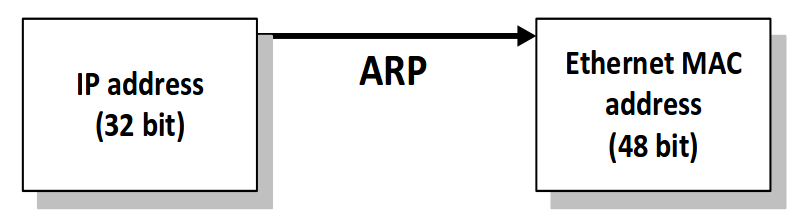
\includegraphics[width=250pt]{../imgs/IPtoMAC.png}
%\caption{Formato de una ARP.}
\end{center}
\end{figure}

Los dos tipos de paquetes posibles en dicho protocolo son los paquetes de petición y de respuesta:
\begin{itemize}
\item Los paquetes de petición ($who-has$) son enviados mayormente en forma de broadcast con el objetivo de poder localizar la dirección MAC a la cual le pertenece una IP conocida.
\item Los paquetes de respuesta ($is-at$) son enviados de manera unicast pues se utilizan para responder a la máquina que realizó una petición con anterioridad.
\end{itemize}

Los paquetes ARP consisten de los siguientes campos:
\begin{itemize}
\item Operación: Especifica la operación que el emisor está realizando. 1 para petición, 2 para responder.
\item Dirección MAC del emisor.
\item Dirección IP del emisior.
\item Dirección MAC del destinatario: Este campo se ignora en las peticiones.
\item Dirección IP del destinatario.
\end{itemize}
\begin{figure}[H] %[h] Aqui [b] para button [t] para top
\begin{center}
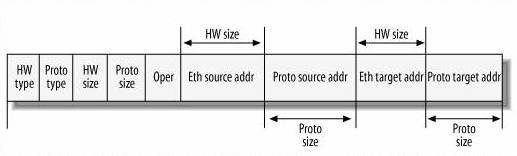
\includegraphics[width=350pt]{../imgs/arp.jpg}
\caption{Formato de una ARP.}
\end{center}
\end{figure}

Un ejemplo típico de uso podría ser el siguiente:

\begin{quotation}
Una máquina en una red desea enviarle un paquete de datos a otra máquina de la misma red. Para eso, la máquina emisora busca, en su tabla local, la dirección MAC asociada a la dirección IP a la cuál desea mandar el paquete. Si no la encuentra, realiza el broadcast de la petición ARP, que llegará eventualmente si se encuentra conectada, a la máquina destino. 
La máquina destino recibirá la petición y responderá de manera unicast a la máquina que realizó la petición, poniendo en el paquete su dirección MAC para que la máquina destino de la respuesta pueda conocer la dirección MAC que necesitaba.
\end{quotation}

El análisis de la red consiste en reconocer su topología en base al nivel de información que proveen las diferentes IP, como fuente y como destino, tomando a las IP como símbolos y estimado su probabilidad de aparición con su frecuencia muestral. Para nuestro análisis, nos limitamos a la utilización de los paquetes $who-has$.

\section{Desarrollo}

Con el fin de obtener resultados relevantes, decidimos analizar redes Wi-Fi públicas de gran uso. Éstas fueron:

\begin{itemize}
\item CECEN-Wifi - Red pública del Pabellón II de Ciudad Universitaria, de gran utilización por parte de los estudiantes y docentes de la facultad.
\item Starbucks Núñez - Red pública utilizada por los clientes.
\item Red Empresarial - Con una magnitud aproximada de 30 dispositivos conectados en simultáneo.
\end{itemize}

Los tiempos de captura fueron los siguientes:

\begin{center}
  \begin{tabular}{| l | c |}
    \hline
    CECEN-Wifi & 23 minutos\\ \hline
    Starbucks & 30 minutos\\ \hline
    Red Empresarial & 30 minutos\\
    \hline
  \end{tabular}
\end{center}

Para la captura de paquetes, generamos un script en Python que, a partir de la biblioteca Scapy\footnote{http://www.secdev.org/projects/scapy/}, $sniffeara$ la red y almacenara las IP's fuente y destino involucradas en el envío y recepción de paquetes. Para corroborar la correctitud de nuestros datos, utilizamos Wireshark\footnote{http://www.wireshark.org} y comparamos lo obtenido con los resultados del programa. 
Las capturas se realizaron seteando la interfaz de red en modo $promiscuo$. Esto significa que vamos a poder analizar paquetes que esten dirigidos a MACs ajenas, y además solo vamos a analizar paquetes de la red en la que estamos asociados mediante el Access Point.

Para almacenar los resultados, filtramos por redes ARP y $who-has$. Los resultados obtenidos fueron los siguientes:

\section{Resultados}

Para cada red consideramos las fuentes de información $S_{src}$ y $S_{dst}$ tales que sus símbolos son las direcciones IP que aparecen como origen y destino en los paquetes ARP \textit{who-has}, respectivamente. Para cada fuente, calculamos la información de cada símbolo\footnote{Es decir, cada dirección IP asociada a esa fuente de información.} utilizando un script.

Con el fin de visualizar los intercambios de paquetes obtenidos, utilizamos $yED$\footnote{http://www.yworks.com/en/products\_yed\_about.html} para realizar gráficos adecuados para ello. Para esto, decidimos presentarlos en forma de grafos dirigidos de IPs con pesos en los nodos (donde existe un eje entre la IP $x$ y la IP $y$ sí y sólo sí se observó un request ARP con source IP $x$ y target IP $y$). Para eso, modificamos su formato obtenido al formato $IP_{src}\ IP_{dst}$ y realizamos los grafos donde el tamaño y el color de cada nodo es proporcional a la cantidad de aristas que lo inciden.

Por otro lado, realizamos gráficos de barra respecto de la entropía. De este modo, logramos analizar qué IPs son estadísticamente significativas en la LAN analizando la información de cada símbolo con respecto a la entropía de su respectiva fuente. Para una simple visualización de los resultados, agregamos el valor de la entropía en forma de recta.

A continuación intentamos identificar los routers en la red utilizando la información de cada IP para ambas fuentes $S_{src}$ y $S_{dst}$. Según suponemos, las IP asociadas a los routers deberían poseer la menor cantidad de información debido a que su frecuencia de recepción e incluso emisión de paquetes ARP debería ser la más alta. Esta suposición se basa en que el router será el dispositivo a los que todos los equipos querrán comunicarse (para poder tener acceso a internet), y mantendrán su ubicación actualizada para poder realizar la comunicación.

Los resultados obtenidos fueron los siguientes:

\subsection{CECEN-Wifi}

La red del $CECEN$ fue capturada durante 23 minutos. Los intercambios que se realizaron en ese tiempo fueron los que se pueden ver a continuación:
\begin{figure}[H] %[h] Aqui [b] para button [t] para top
\begin{center}
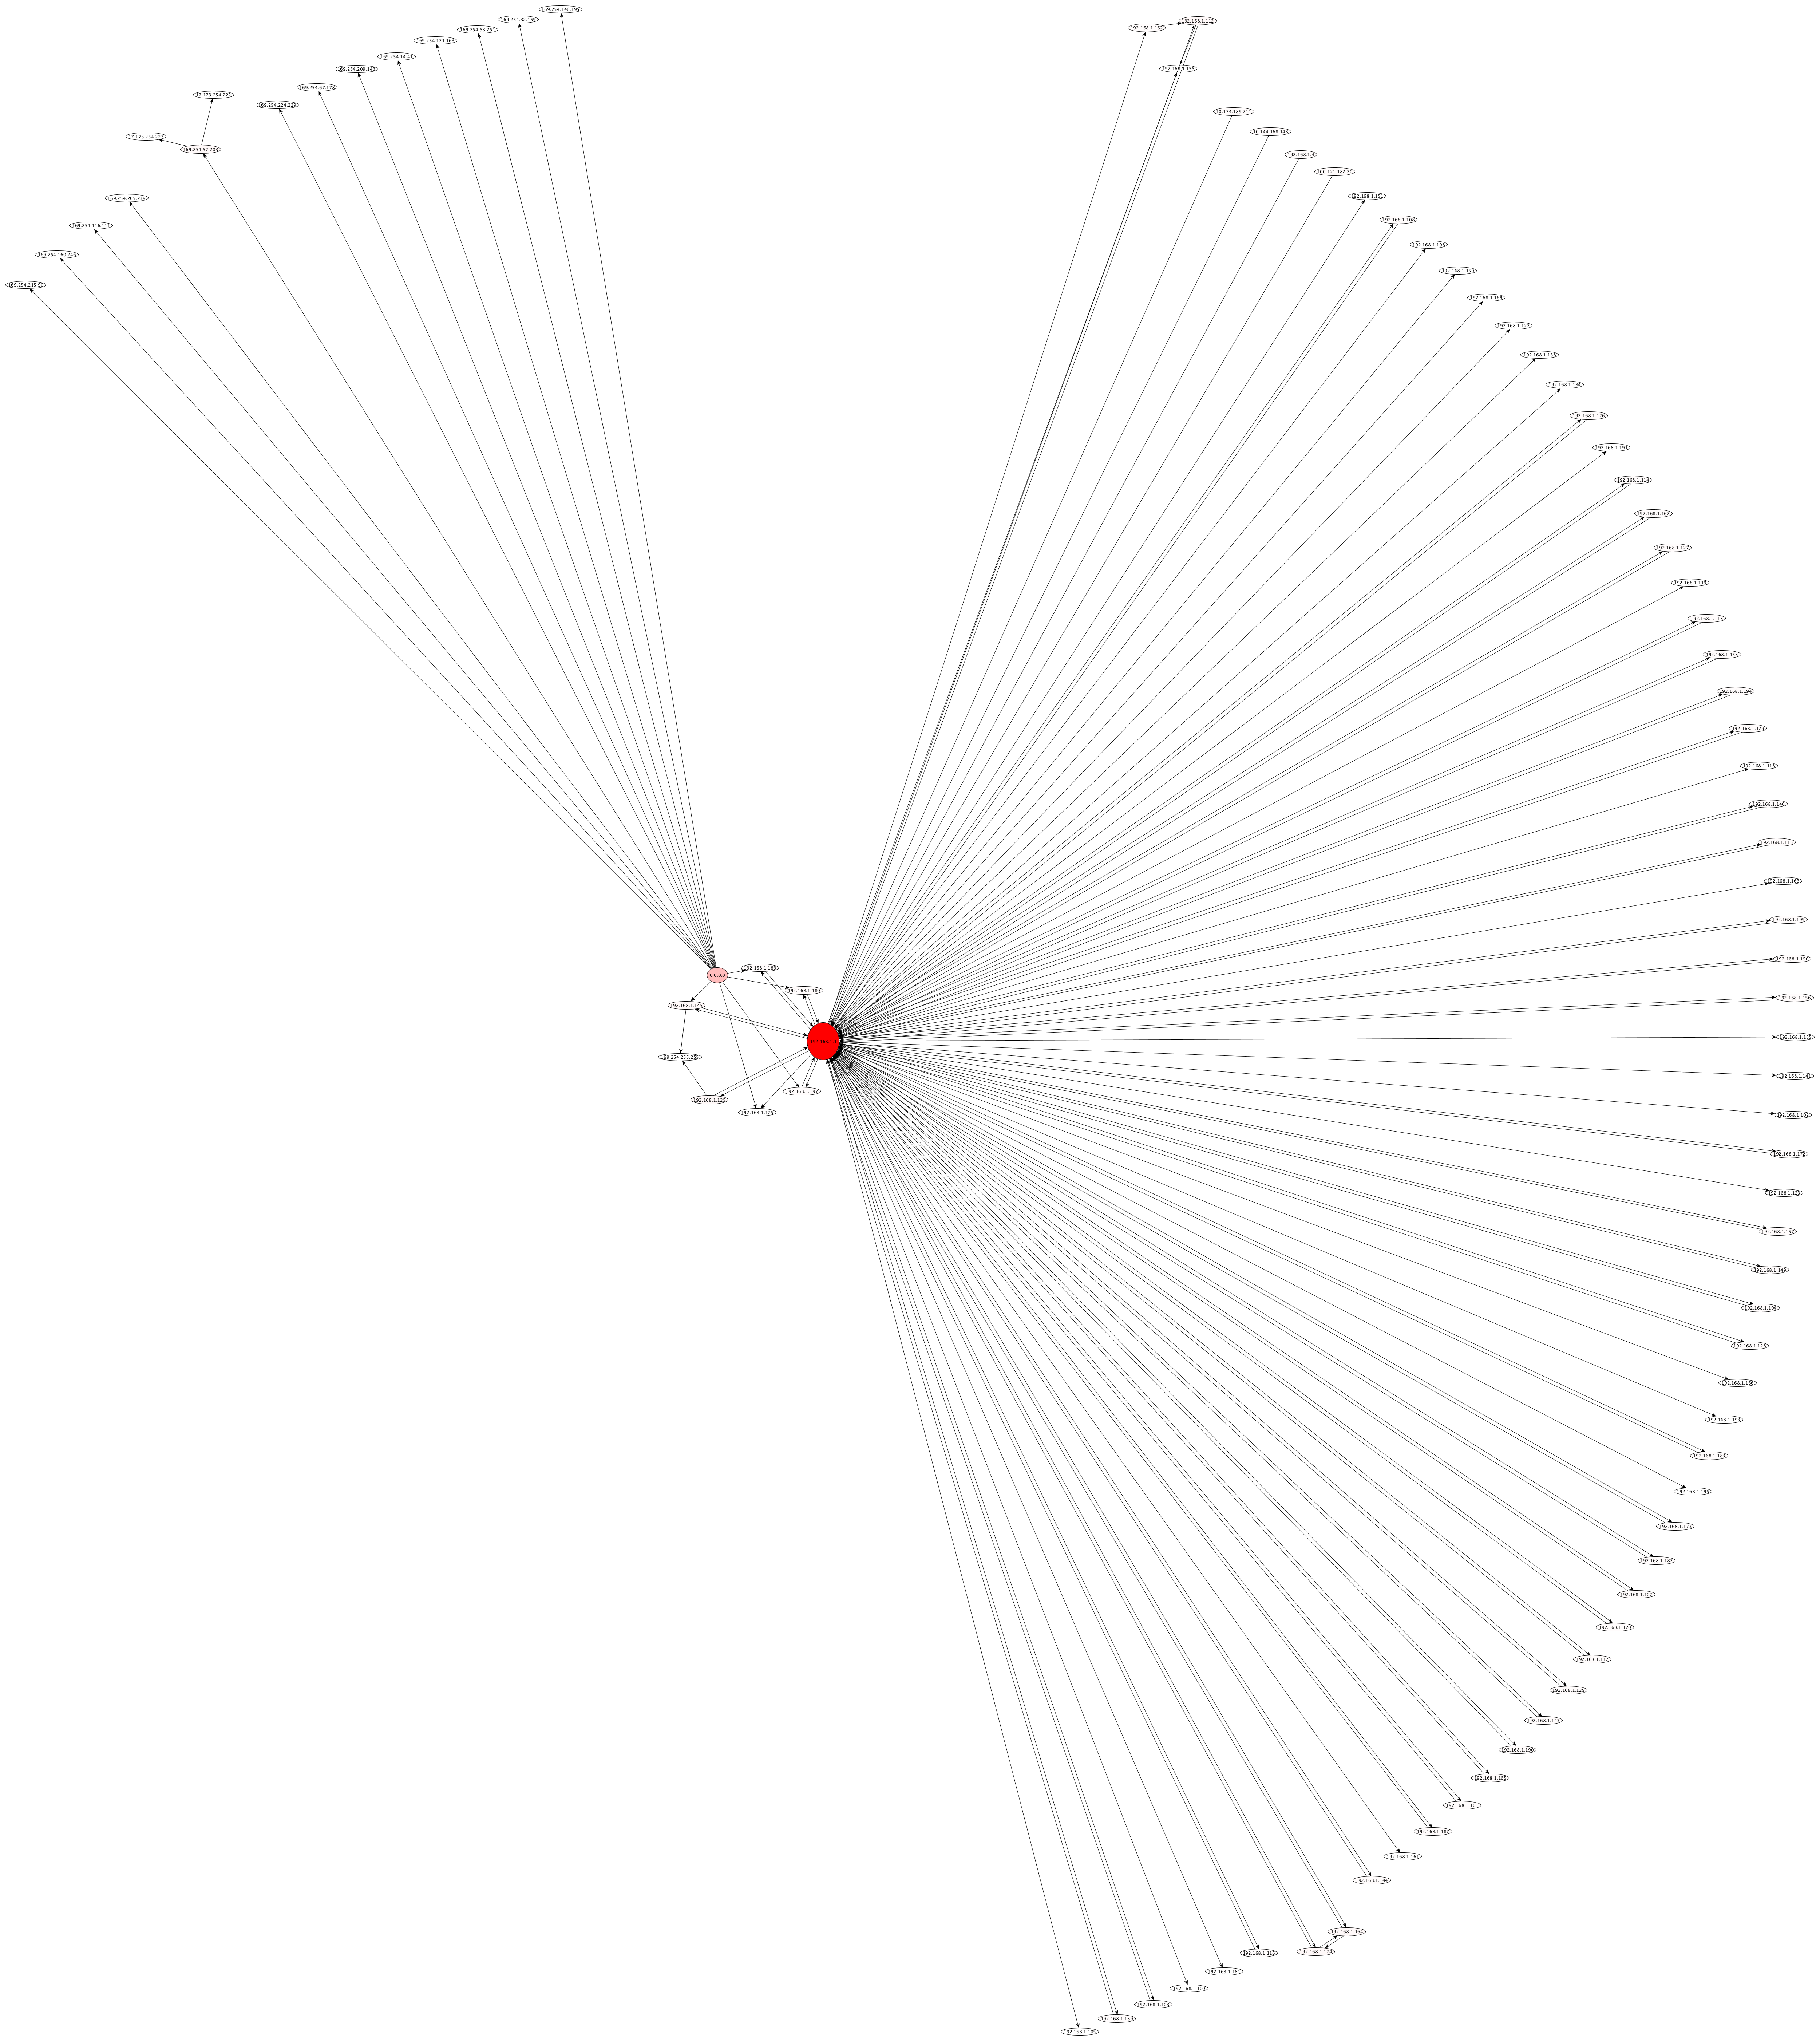
\includegraphics[width=450pt]{../imgs/cecen-outgoing.png}
\caption{Resultado de la captura de Outgoing de paquetes de la red CECEN-Wifi.}
\end{center}
\end{figure}

\begin{figure}[H] %[h] Aqui [b] para button [t] para top
\begin{center}
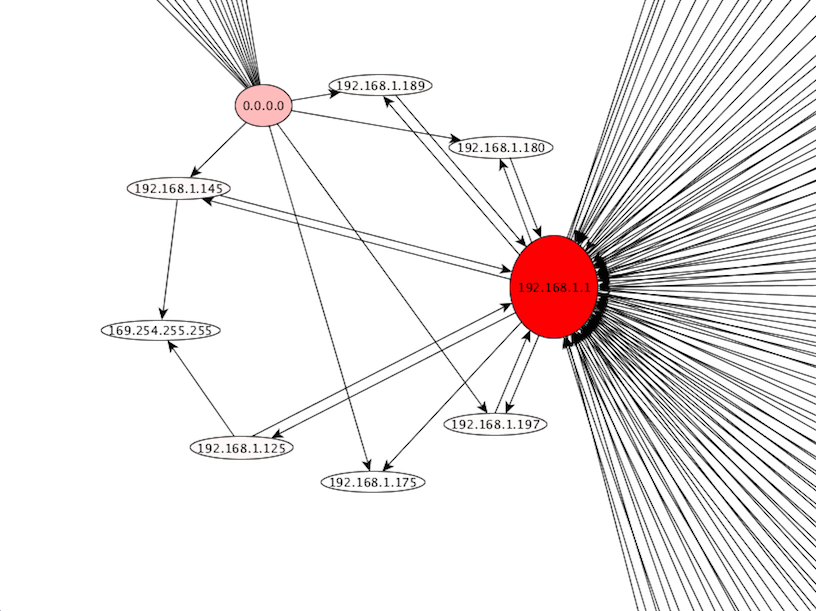
\includegraphics[width=400pt]{../imgs/zoom-cecen-outgoing.png}
\caption{Zoom de la captura de Outgoing de paquetes de la red CECEN-Wifi.}
\end{center}
\end{figure}

Como se puede observar, el router que actúa como $gateway$ es la IP 192.168.1.1 dado que se encuentra representada por el nodo de mayor tamaño y color más oscuro. En este caso, la segunda IP con mayor cantidad de envío de paquetes es 0.0.0.0.


\begin{figure}[H] %[h] Aqui [b] para button [t] para top
\begin{center}
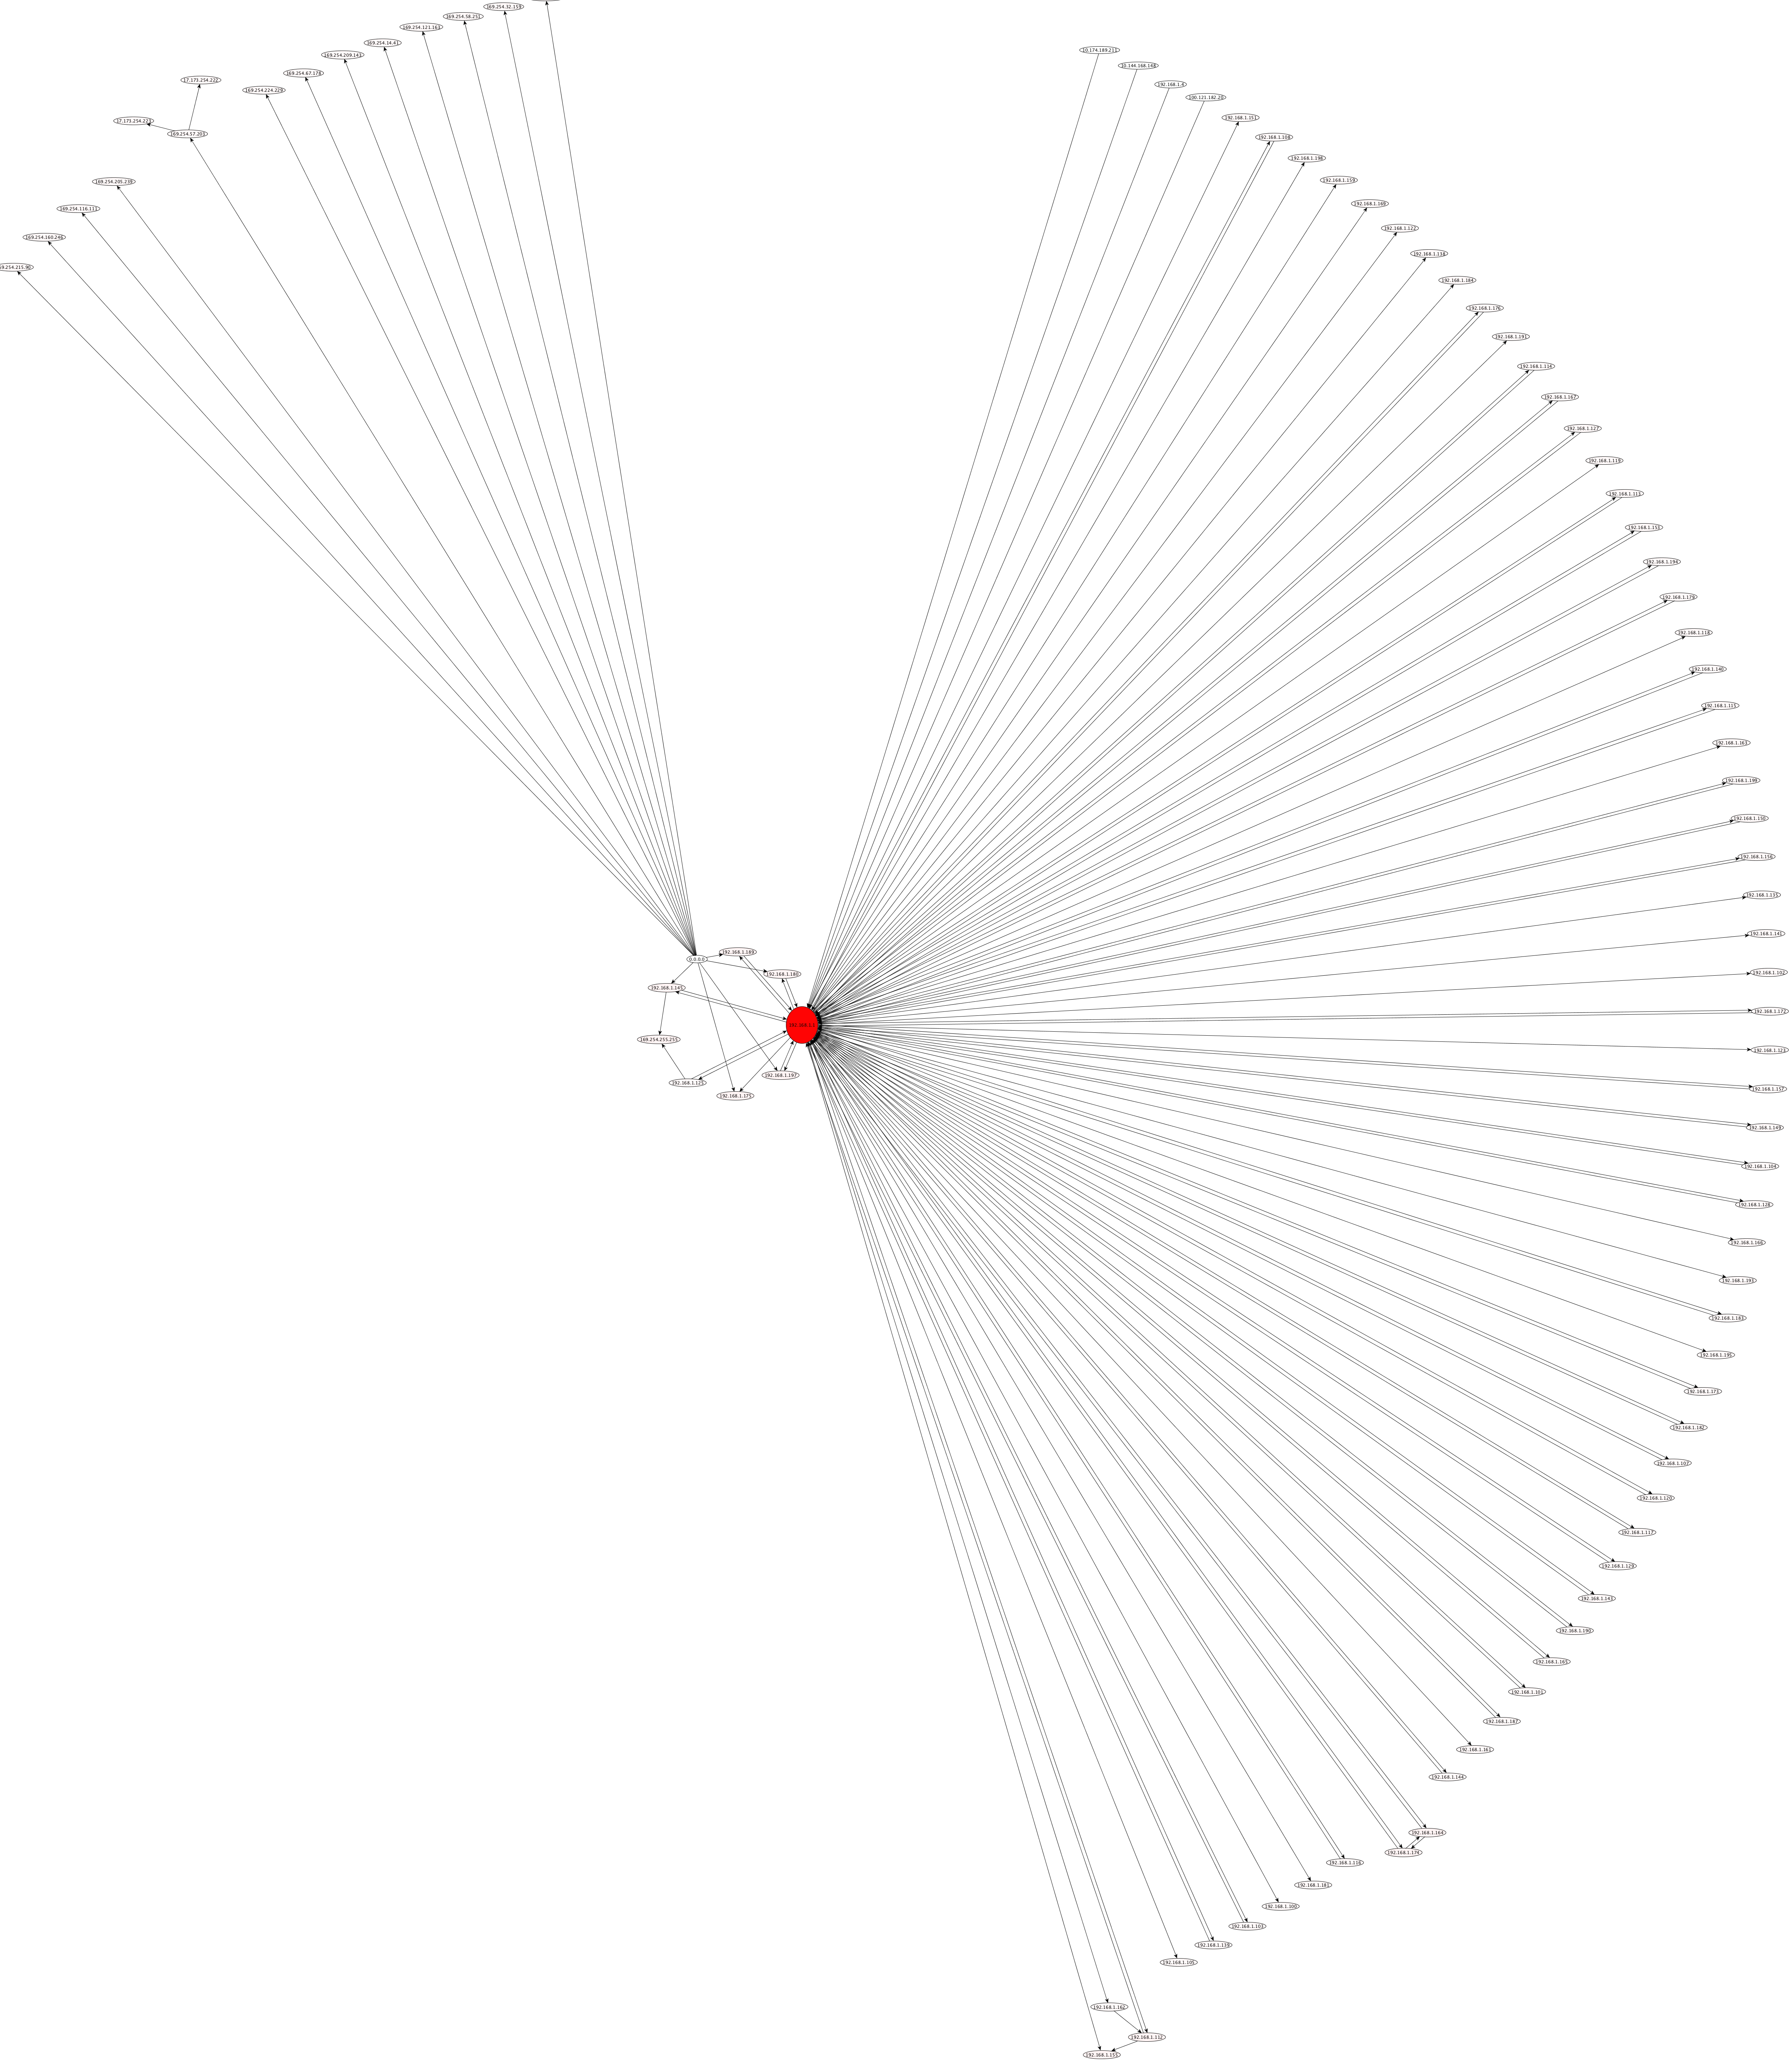
\includegraphics[width=450pt]{../imgs/cecen-incoming.png}
\caption{Resultado de la captura de Incoming de paquetes de la red CECEN-Wifi.}
\end{center}
\end{figure}

\begin{figure}[H] %[h] Aqui [b] para button [t] para top
\begin{center}
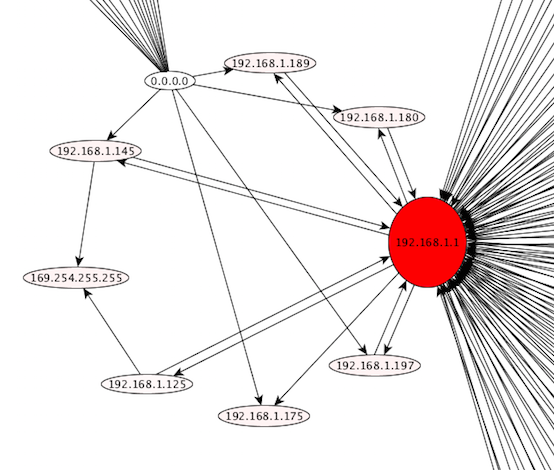
\includegraphics[width=400pt]{../imgs/zoom-cecen-incoming.png}
\caption{Zoom de la captura de Incoming de paquetes de la red CECEN-Wifi.}
\end{center}
\end{figure}

Como se puede observar, el router que actúa como $gateway$ es la IP 192.168.1.1 dado que se encuentra representada por el nodo de mayor tamaño y color más oscuro. El resto de las IPs presentan tamaño y color similares, luego no hay ninguna cuya cantidad de aristas que las inciden sean relevantes respecto de las demás.

\begin{figure}[H] %[h] Aqui [b] para button [t] para top
\begin{center}
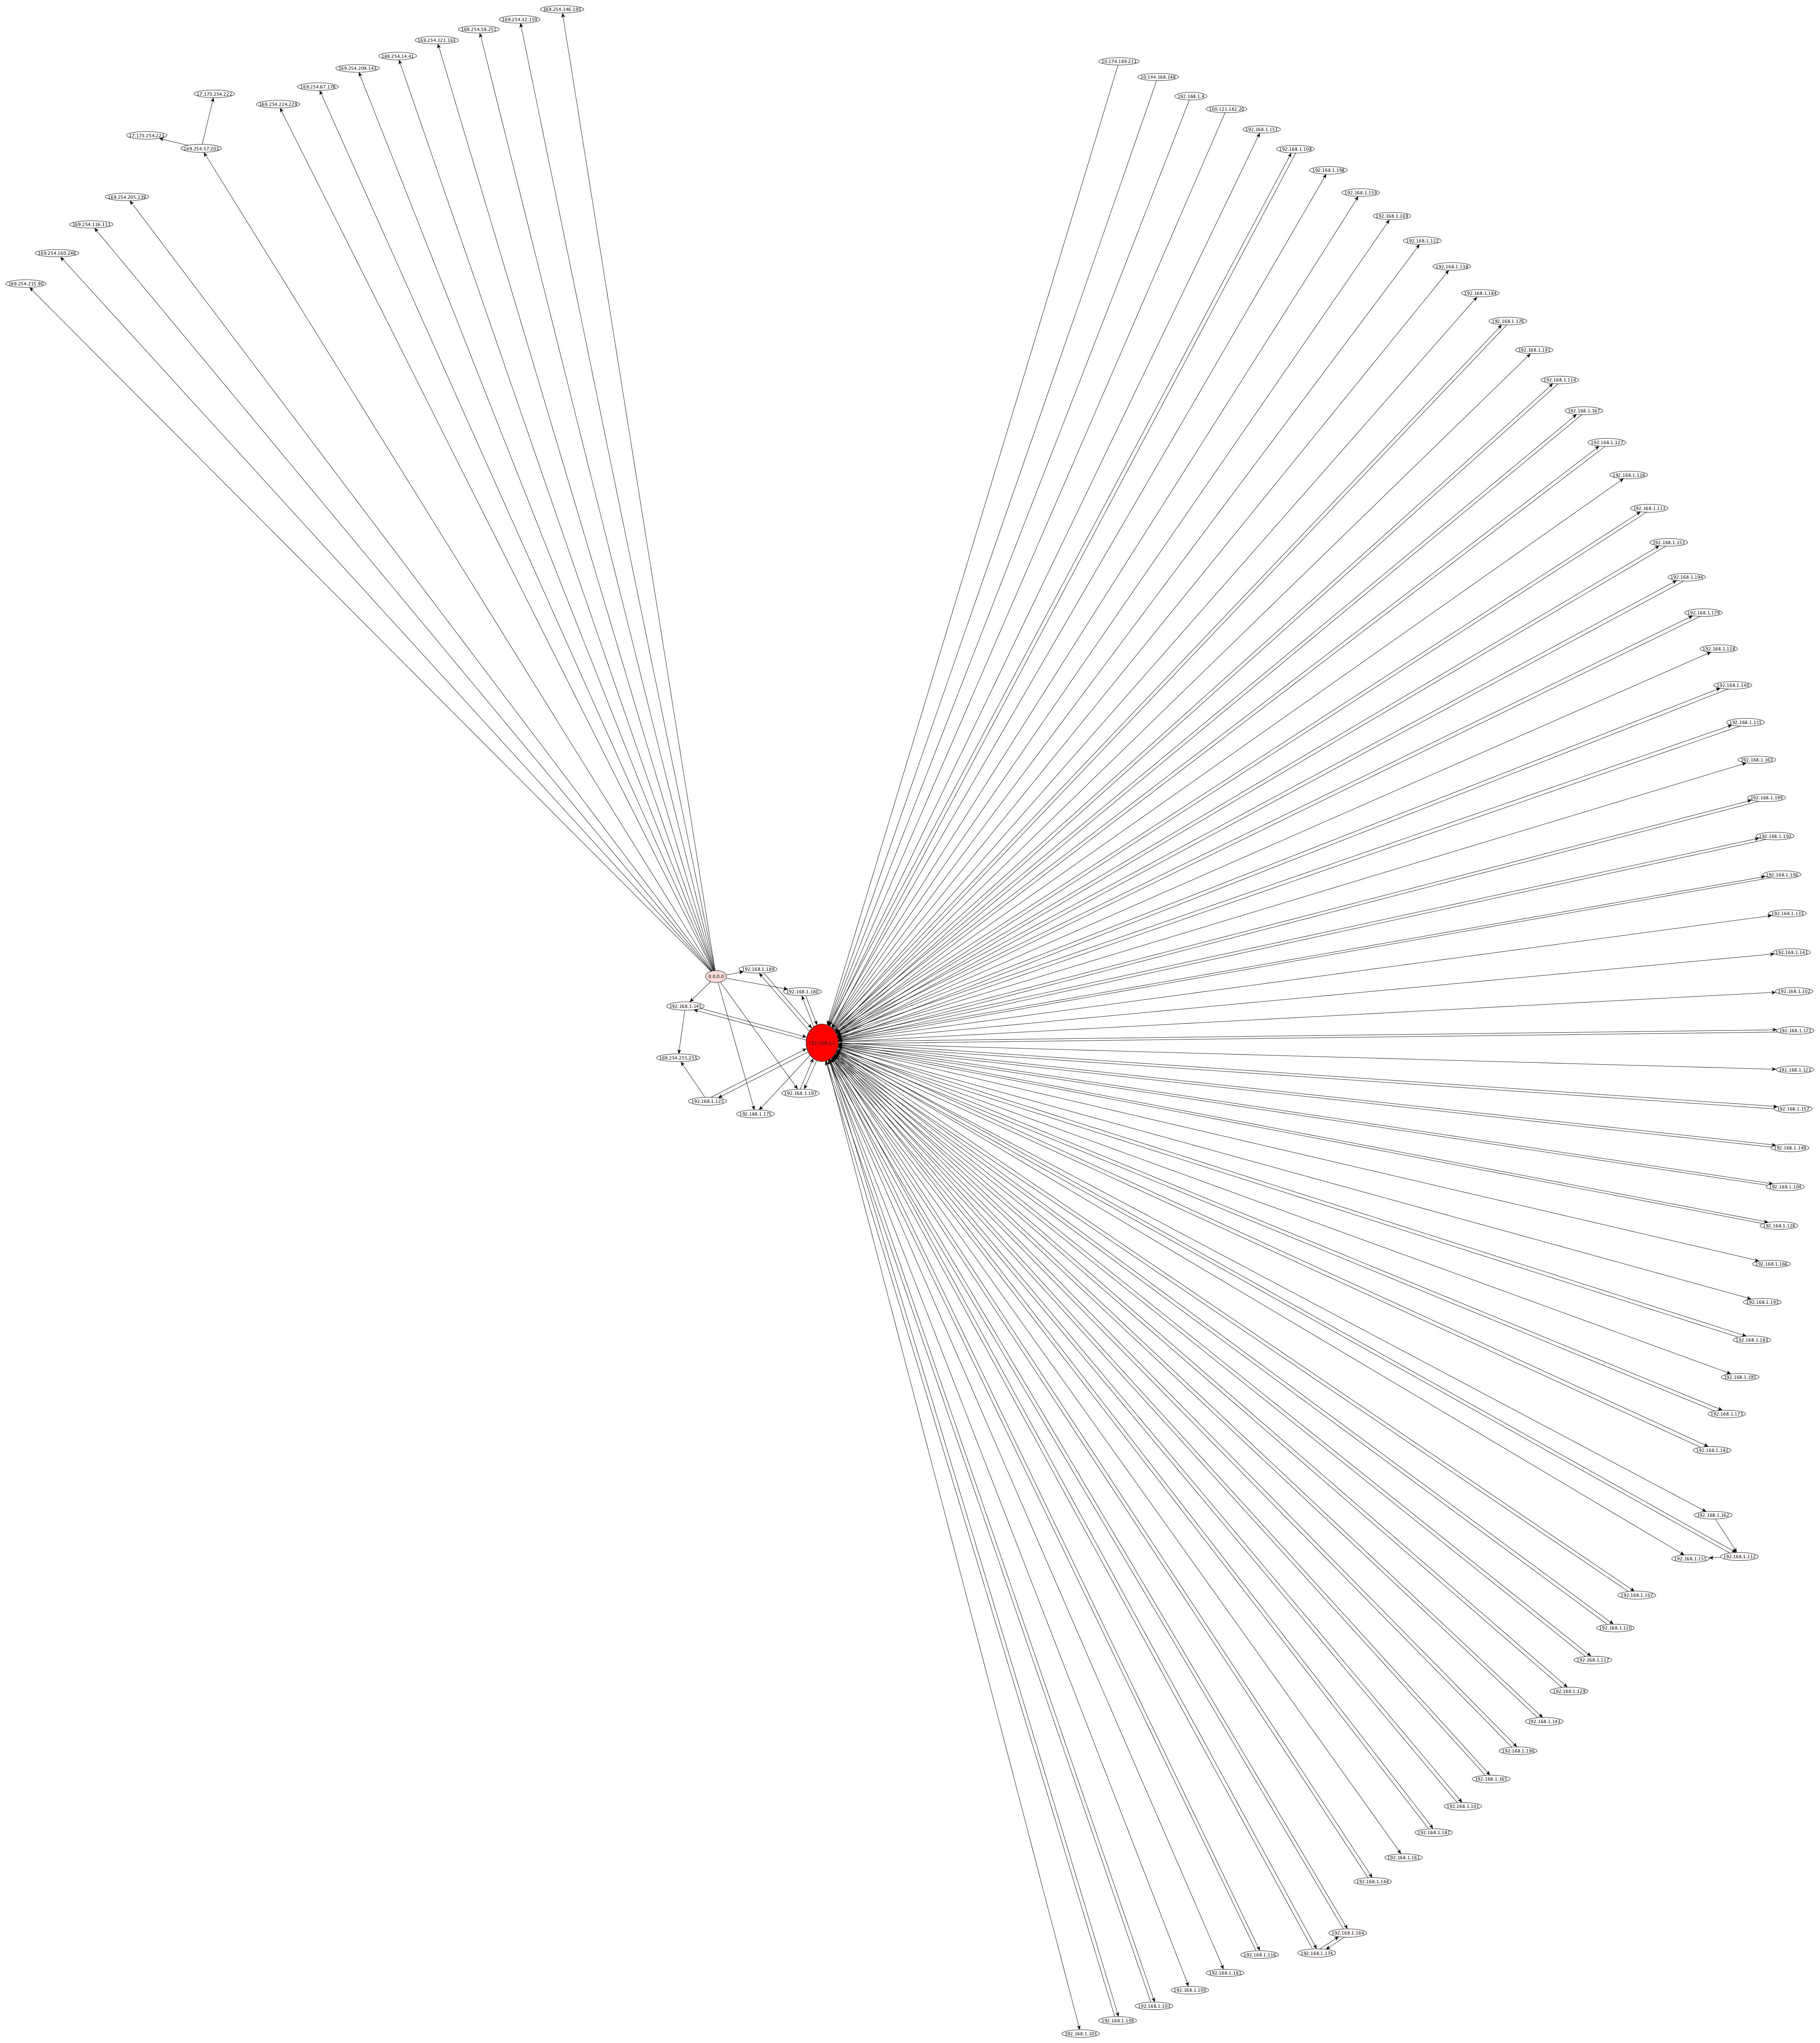
\includegraphics[width=450pt]{../imgs/cecen-entero.png}
\caption{Resultado de la captura de envío y recepción (Incoming+Outgoing) de paquetes de la red CECEN-Wifi.}
\end{center}
\end{figure}

Como se puede observar, los tres grafos son isomorfos. Esto se debe a que la mayoría de los dispositivos que envían datos también reciben. Dado que el router es el que más envía y recibe paquetes comunicándose con todos los demás dispositivos, es el de mayor tamaño y color más oscuro en las tres representaciones.

\subsubsection{Información de la fuente}

A continuación se muestran las 10 IPs con menor cantidad de información.

\begin{itemize}

\item \textbf{Fuente src}
\begin{figure}[H] %[h] Aqui [b] para button [t] para top
\begin{center}
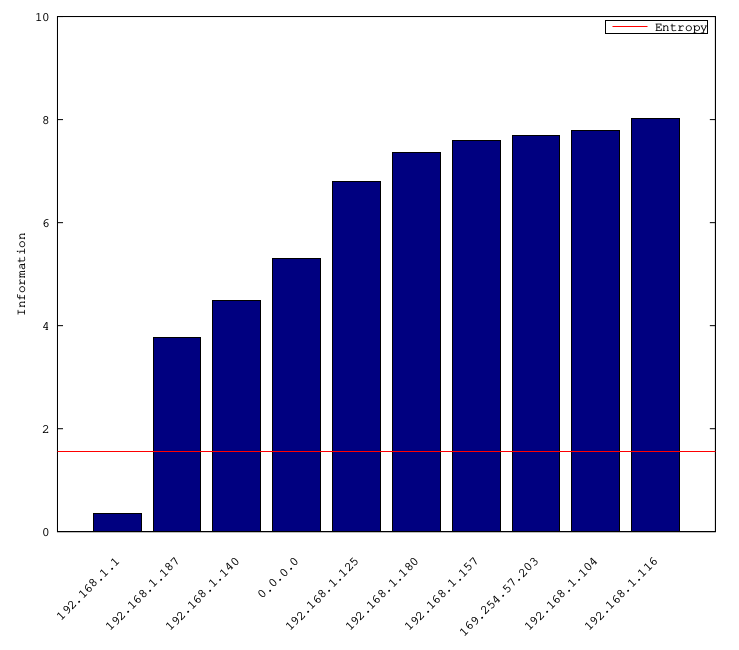
\includegraphics[width=400pt]{../imgs/cecen_src_chartbar.png}
\caption{Información de los símbolos(IPs) origen.}
\end{center}
\end{figure}

\item \textbf{Fuente dst}

\begin{figure}[H] %[h] Aqui [b] para button [t] para top
\begin{center}
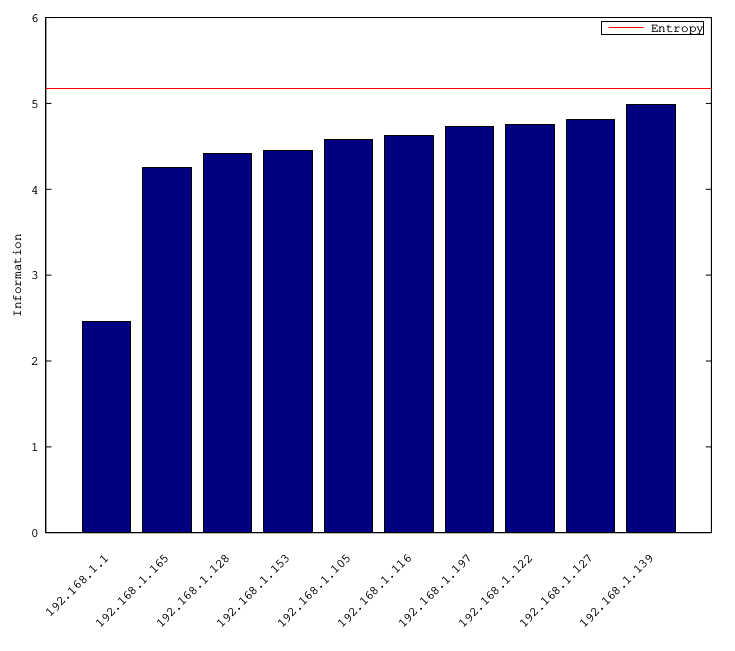
\includegraphics[width=400pt]{../imgs/cecen_dst_chartbar.png}
\caption{Información de los símbolos(IPs) destino.}
\end{center}
\end{figure}
\end{itemize}

Luego del análisis de grafos representados en la sección de arriba, se puede observar que la IP con menor cantidad de información es la 192.168.1.1. Esto resulta lógico dado que consiste en la IP del router, encargado de la transferencia de la mayor cantidad de paquetes con todos los dispositivos conectados a la red. Dado que la amplitud de transferencia de paquetes es similar en el resto de los dispositivos, su cantidad de información es semejante.

\subsection{Starbucks}

 El resultado de capturar durante 30 minutos la red de Starbucks fue el que sigue:

\begin{figure}[H] %[h] Aqui [b] para button [t] para top
\begin{center}
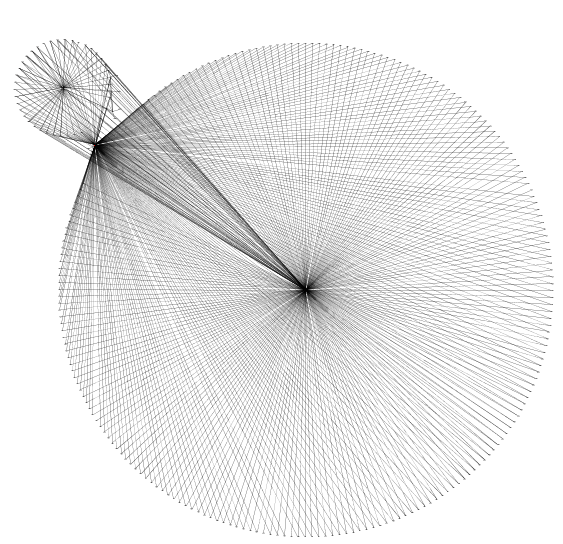
\includegraphics[width=450pt]{../imgs/starbucks30_entero.png}
\caption{Resultado de la captura de envío y recepción de paquetes de Starbucks durante 30 minutos.}
\end{center}
\end{figure}

Como se puede observar, son dos las direcciones IP que realizan intercambios con el resto de los dispositivos conectados a la red, luego las que funcionan como gateways. Una de ellas es el router y la otra, un celular que se utilizó para evaluar los dispositivos conectados a la red a través de la aplicación $Fing\ -\ Network Tools$ \footnote{$play.google.com/store/apps/details?id=com.overlook.android.fing\&hl=fr$}. Dicha aplicación encuentra las redes Wi-Fi conectadas en tiempo real, evaluando niveles de seguridad y mostrando las direcciones MAC de cada dispositivo conectado como también su fabricante. Utilizamos dicha aplicación para evaluar las modificaciones que podían surgir en el intercambio de paquetes y consideramos interesante variar el análisis.

\begin{figure}[H] %[h] Aqui [b] para button [t] para top
\begin{center}
\includegraphics[width=450pt]{../imgs/starbucks30-incoming.png}
\caption{Resultado de la captura de Incoming de paquetes de Starbucks durante 30 minutos.}
\end{center}
\end{figure}

\begin{figure}[H] %[h] Aqui [b] para button [t] para top
\begin{center}
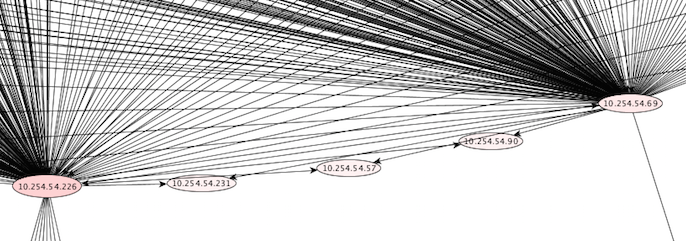
\includegraphics[width=450pt]{../imgs/zoom-starbucks-incoming.png}
\caption{Zoom de la captura de Incoming de paquetes de Starbucks durante 30 minutos.}
\end{center}
\end{figure}

\begin{figure}[H] %[h] Aqui [b] para button [t] para top
\begin{center}
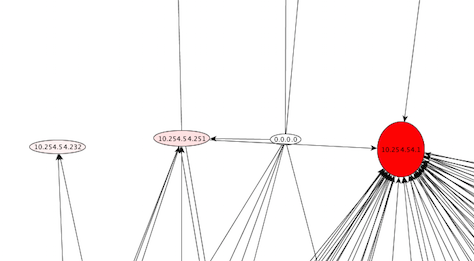
\includegraphics[width=450pt]{../imgs/zoom-starbucks-incoming2.png}
\caption{Zoom de la captura de Incoming de paquetes de Starbucks durante 30 minutos.}
\end{center}
\end{figure}


\begin{figure}[H] %[h] Aqui [b] para button [t] para top
\begin{center}
\includegraphics[width=450pt]{../imgs/starbucks30-outgoing.png}
\caption{Resultado de la captura de Outgoing de paquetes de Starbucks durante 30 minutos.}
\end{center}
\end{figure}

\begin{figure}[H] %[h] Aqui [b] para button [t] para top
\begin{center}
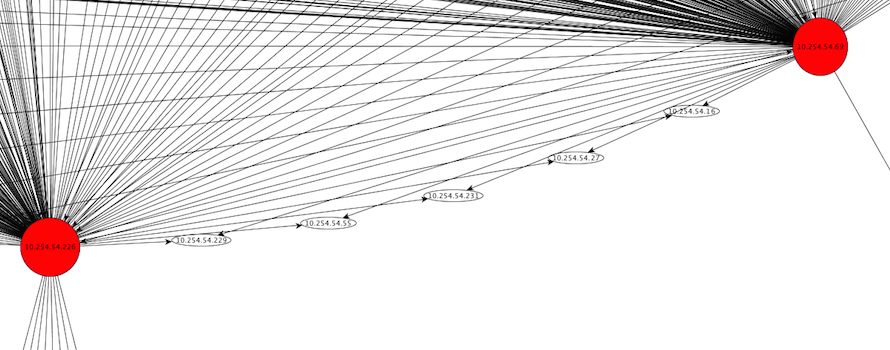
\includegraphics[width=450pt]{../imgs/zoom-starbucks-outgoing.png}
\caption{Zoom de la captura de Outgoing de paquetes de Starbucks durante 30 minutos.}
\end{center}
\end{figure}

\begin{figure}[H] %[h] Aqui [b] para button [t] para top
\begin{center}
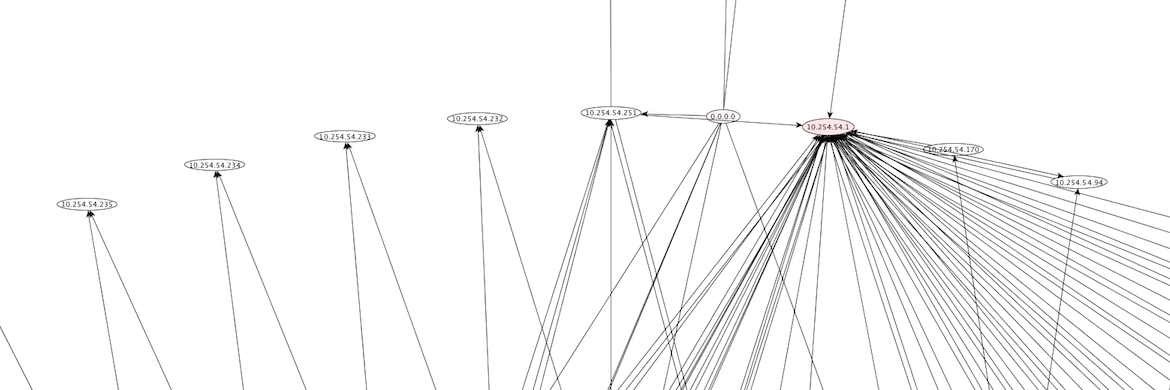
\includegraphics[width=450pt]{../imgs/zoom-starbucks-outgoing2.png}
\caption{Zoom de la captura de Outgoing de paquetes de Starbucks durante 30 minutos.}
\end{center}
\end{figure}

\subsubsection{Información de la fuente}

A continuación se muestran las 10 IPs con menor cantidad de información.

\begin{itemize}
\item \textbf{Fuente src}

\begin{figure}[H] %[h] Aqui [b] para button [t] para top
\begin{center}
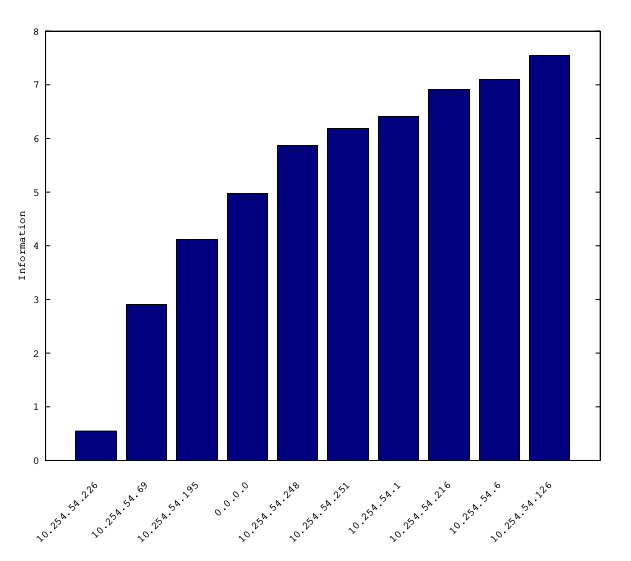
\includegraphics[width=400pt]{../imgs/starbucks_src_chartbar.png}
\caption{Información de los símbolos(IPs) origen.}
\end{center}
\end{figure}

\item \textbf{Fuente dst}

\begin{figure}[H] %[h] Aqui [b] para button [t] para top
\begin{center}
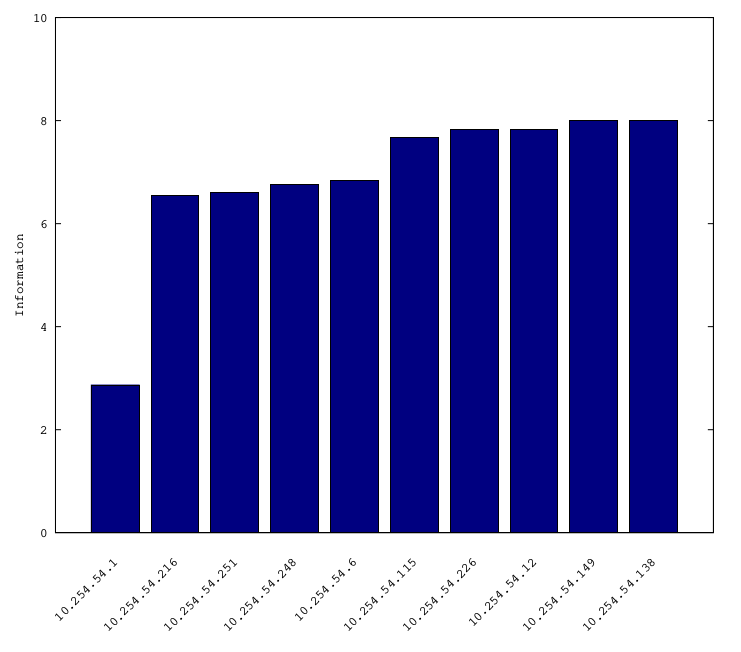
\includegraphics[width=400pt]{../imgs/starbucks_dst_chartbar.png}
\caption{Información de los símbolos(IPs) destino.}
\end{center}
\end{figure}

\end{itemize}

\subsection{Red Empresarial}

\begin{figure}[H] %[h] Aqui [b] para button [t] para top
\begin{center}
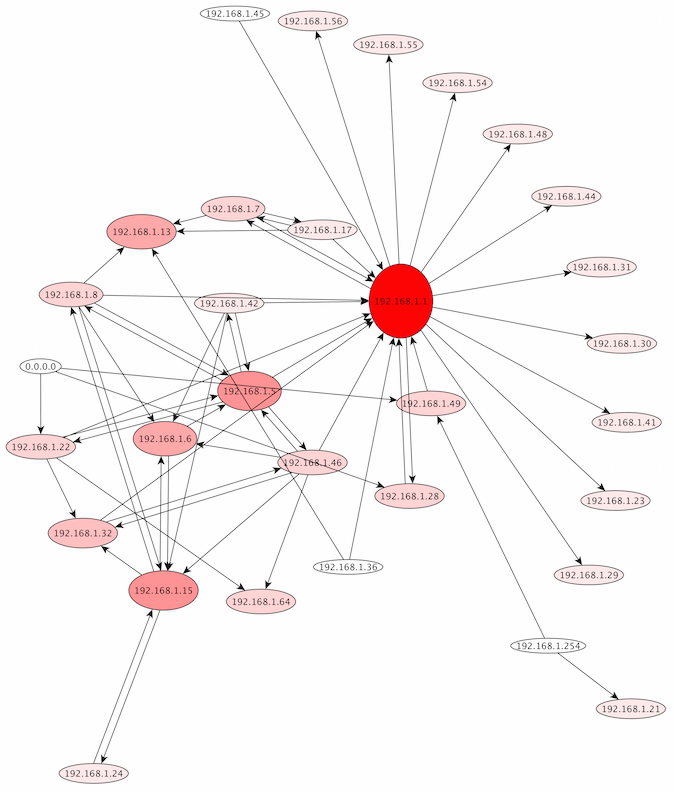
\includegraphics[width=400pt]{../imgs/tiarg-incoming.png}
\caption{Resultado de la captura Incoming de paquetes de una empresa.}
\end{center}
\end{figure}

\begin{figure}[H] %[h] Aqui [b] para button [t] para top
\begin{center}
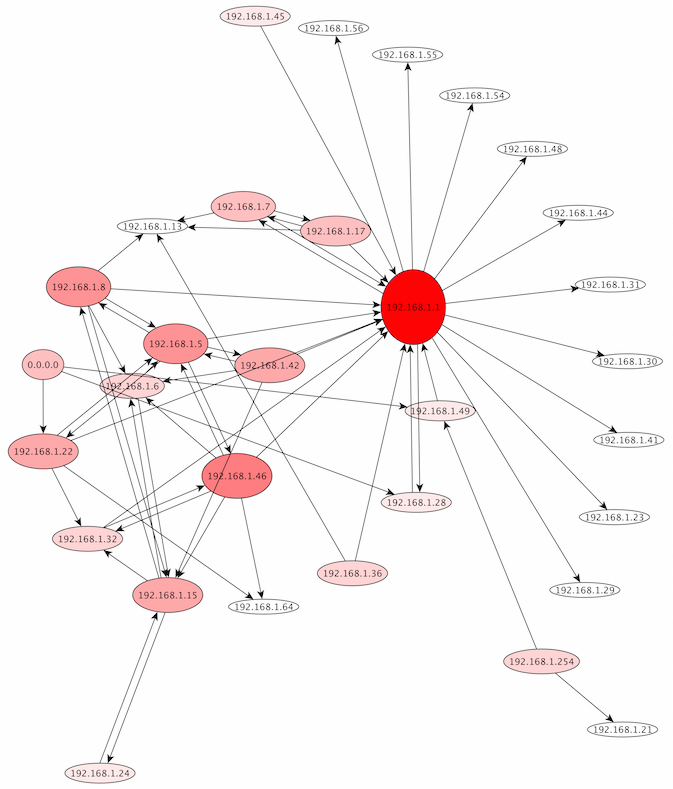
\includegraphics[width=400pt]{../imgs/tiarg-outgoing.png}
\caption{Resultado de la captura de Outgoing de paquetes de una empresa.}
\end{center}
\end{figure}

Como se puede observar, el router que actúa como $gateway$ es la IP 192.168.1.1.

\subsubsection{Información de la fuente}

A continuación se muestran las 10 IPs con menor cantidad de información.

\begin{itemize}
\item \textbf{Fuente src}

\begin{figure}[H] %[h] Aqui [b] para button [t] para top
\begin{center}
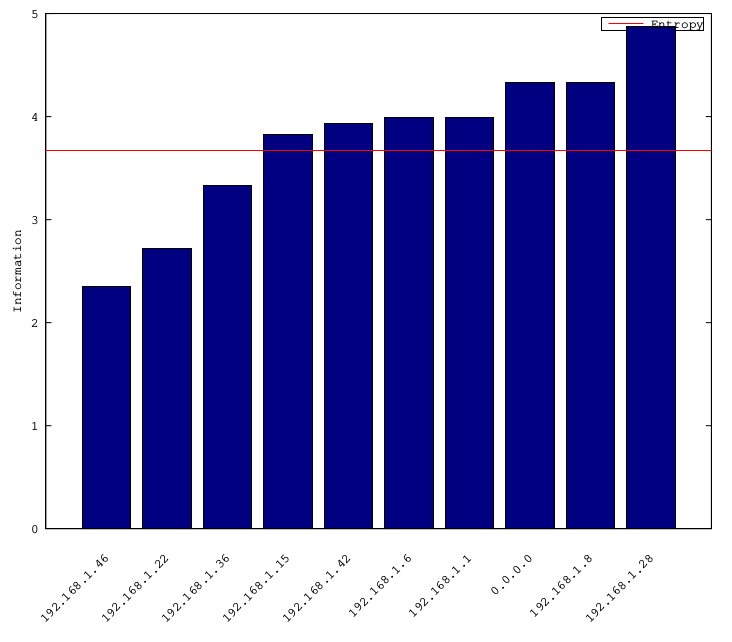
\includegraphics[width=400pt]{../imgs/tiarg_src_chartbar.png}
\caption{Información de los símbolos(IPs) origen.}
\end{center}
\end{figure}

\item \textbf{Fuente dst}

%% GNUPLOT: LaTeX picture with Postscript
\begingroup
  \makeatletter
  \providecommand\color[2][]{%
    \GenericError{(gnuplot) \space\space\space\@spaces}{%
      Package color not loaded in conjunction with
      terminal option `colourtext'%
    }{See the gnuplot documentation for explanation.%
    }{Either use 'blacktext' in gnuplot or load the package
      color.sty in LaTeX.}%
    \renewcommand\color[2][]{}%
  }%
  \providecommand\includegraphics[2][]{%
    \GenericError{(gnuplot) \space\space\space\@spaces}{%
      Package graphicx or graphics not loaded%
    }{See the gnuplot documentation for explanation.%
    }{The gnuplot epslatex terminal needs graphicx.sty or graphics.sty.}%
    \renewcommand\includegraphics[2][]{}%
  }%
  \providecommand\rotatebox[2]{#2}%
  \@ifundefined{ifGPcolor}{%
    \newif\ifGPcolor
    \GPcolorfalse
  }{}%
  \@ifundefined{ifGPblacktext}{%
    \newif\ifGPblacktext
    \GPblacktexttrue
  }{}%
  % define a \g@addto@macro without @ in the name:
  \let\gplgaddtomacro\g@addto@macro
  % define empty templates for all commands taking text:
  \gdef\gplbacktext{}%
  \gdef\gplfronttext{}%
  \makeatother
  \ifGPblacktext
    % no textcolor at all
    \def\colorrgb#1{}%
    \def\colorgray#1{}%
  \else
    % gray or color?
    \ifGPcolor
      \def\colorrgb#1{\color[rgb]{#1}}%
      \def\colorgray#1{\color[gray]{#1}}%
      \expandafter\def\csname LTw\endcsname{\color{white}}%
      \expandafter\def\csname LTb\endcsname{\color{black}}%
      \expandafter\def\csname LTa\endcsname{\color{black}}%
      \expandafter\def\csname LT0\endcsname{\color[rgb]{1,0,0}}%
      \expandafter\def\csname LT1\endcsname{\color[rgb]{0,1,0}}%
      \expandafter\def\csname LT2\endcsname{\color[rgb]{0,0,1}}%
      \expandafter\def\csname LT3\endcsname{\color[rgb]{1,0,1}}%
      \expandafter\def\csname LT4\endcsname{\color[rgb]{0,1,1}}%
      \expandafter\def\csname LT5\endcsname{\color[rgb]{1,1,0}}%
      \expandafter\def\csname LT6\endcsname{\color[rgb]{0,0,0}}%
      \expandafter\def\csname LT7\endcsname{\color[rgb]{1,0.3,0}}%
      \expandafter\def\csname LT8\endcsname{\color[rgb]{0.5,0.5,0.5}}%
    \else
      % gray
      \def\colorrgb#1{\color{black}}%
      \def\colorgray#1{\color[gray]{#1}}%
      \expandafter\def\csname LTw\endcsname{\color{white}}%
      \expandafter\def\csname LTb\endcsname{\color{black}}%
      \expandafter\def\csname LTa\endcsname{\color{black}}%
      \expandafter\def\csname LT0\endcsname{\color{black}}%
      \expandafter\def\csname LT1\endcsname{\color{black}}%
      \expandafter\def\csname LT2\endcsname{\color{black}}%
      \expandafter\def\csname LT3\endcsname{\color{black}}%
      \expandafter\def\csname LT4\endcsname{\color{black}}%
      \expandafter\def\csname LT5\endcsname{\color{black}}%
      \expandafter\def\csname LT6\endcsname{\color{black}}%
      \expandafter\def\csname LT7\endcsname{\color{black}}%
      \expandafter\def\csname LT8\endcsname{\color{black}}%
    \fi
  \fi
  \setlength{\unitlength}{0.0500bp}%
  \begin{picture}(9000.00,4500.00)%
    \gplgaddtomacro\gplbacktext{%
      \colorrgb{0.00,0.00,0.00}%
      \put(500,240){\makebox(0,0)[r]{\strut{}0}}%
      \colorrgb{0.00,0.00,0.00}%
      \put(500,910){\makebox(0,0)[r]{\strut{}1}}%
      \colorrgb{0.00,0.00,0.00}%
      \put(500,1580){\makebox(0,0)[r]{\strut{}2}}%
      \colorrgb{0.00,0.00,0.00}%
      \put(500,2250){\makebox(0,0)[r]{\strut{}3}}%
      \colorrgb{0.00,0.00,0.00}%
      \put(500,2919){\makebox(0,0)[r]{\strut{}4}}%
      \colorrgb{0.00,0.00,0.00}%
      \put(500,3589){\makebox(0,0)[r]{\strut{}5}}%
      \colorrgb{0.00,0.00,0.00}%
      \put(500,4259){\makebox(0,0)[r]{\strut{}6}}%
      \colorrgb{0.00,0.00,0.00}%
      \put(160,2249){\rotatebox{90}{\makebox(0,0){\strut{}Informaci\'on}}}%
    }%
    \gplgaddtomacro\gplfronttext{%
      \colorrgb{0.00,0.00,0.00}%
      \put(1349,29){\rotatebox{45}{\makebox(0,0)[r]{\strut{}192.168.1.1}}}%
      \put(2078,29){\rotatebox{45}{\makebox(0,0)[r]{\strut{}192.168.1.15}}}%
      \put(2807,29){\rotatebox{45}{\makebox(0,0)[r]{\strut{}192.168.1.32}}}%
      \put(3536,29){\rotatebox{45}{\makebox(0,0)[r]{\strut{}192.168.1.5}}}%
      \put(4265,29){\rotatebox{45}{\makebox(0,0)[r]{\strut{}192.168.1.13}}}%
      \put(4994,29){\rotatebox{45}{\makebox(0,0)[r]{\strut{}192.168.1.6}}}%
      \put(5723,29){\rotatebox{45}{\makebox(0,0)[r]{\strut{}192.168.1.64}}}%
      \put(6452,29){\rotatebox{45}{\makebox(0,0)[r]{\strut{}192.168.1.22}}}%
      \put(7181,29){\rotatebox{45}{\makebox(0,0)[r]{\strut{}192.168.1.29}}}%
      \put(7910,29){\rotatebox{45}{\makebox(0,0)[r]{\strut{}192.168.1.28}}}%
    }%
    \gplbacktext
    \put(0,0){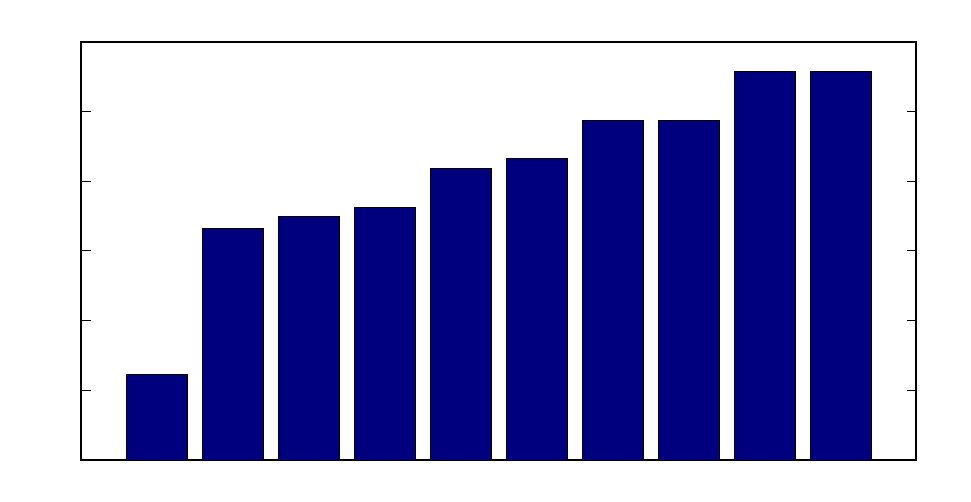
\includegraphics{./imgs/chartBar/tiarg_dst_barchart}}%
    \gplfronttext
  \end{picture}%
\endgroup

\begin{figure}[H] %[h] Aqui [b] para button [t] para top
\begin{center}
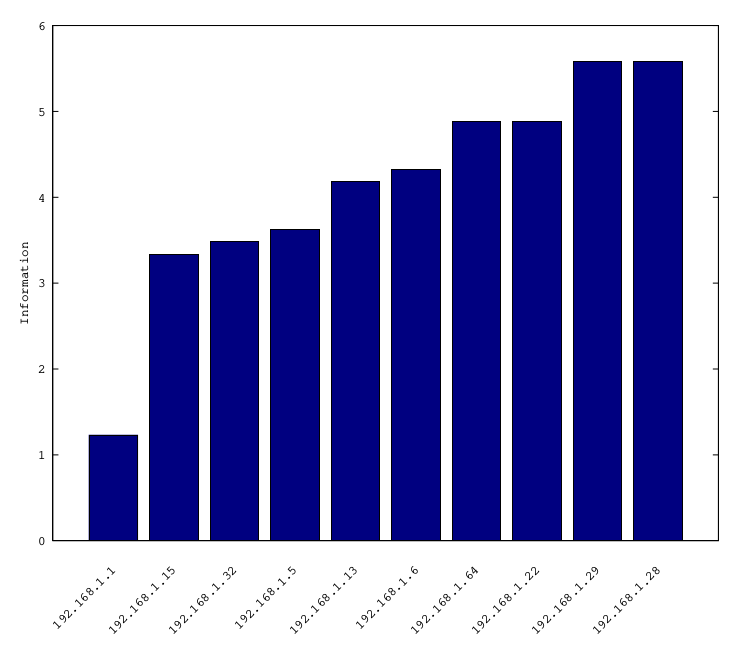
\includegraphics[width=400pt]{../imgs/tiarg_dst_chartbar.png}
\caption{Información de los símbolos(IPs) destino.}
\end{center}
\end{figure}

\end{itemize}


\subsection{Información estadística obtenida de las muestras}

\begin{center}
\begin{tabular}{|c|c|c|}
\hline
Red & Tamaño de la muestra (paquetes)\\
\hline
CECEN-Wifi & 3017 \\
Starbucks   & 2050 \\
Empresa    &  382 \\
\hline
\end{tabular}
\end{center}


\subsubsection{Entropía}

\begin{center}
\begin{tabular}{|c|c|c|}
\hline
Red & Fuente de información modelada $S$ & Entropía $H(S)$\\
\hline
\multirow{2}{*}{CECEN-Wifi}  & $S_{src}$ & 1.56 \\
						     & $S_{dst}$ & 5.17 \\
\hline
\multirow{2}{*}{Starbucks}   & $S_{src}$ & 1.84 \\
						     & $S_{dst}$ & 7.44 \\
\hline
\multirow{2}{*}{Empresa}     & $S_{src}$ & 3.67 \\
						    & $S_{dst}$ & 3.12 \\
\hline
\end{tabular}
\end{center}

\section{Discusión}
Describimos a continuación nuestra interpretación de algunos fenómenos observados, de manera de facilitar la discusión de los resultados obtenidos.

\subsection{Nodos que emiten paquetes ARP \textit{who-has} hacia un único nodo destino}

Dado que la captura de paquetes fue realizada sobre redes wireless públicas, asumimos que la mayoría de las personas conectadas a la red sólo desean obtener acceso a internet, con lo que sus dispositivos únicamente solicitan la dirección física del gateway que les asigna al conectarse a la red.


\subsection{Nodos que emiten paquetes ARP \textit{who-has} hacia muchos nodos destino}

Teniendo en cuenta lo anterior, interpretamos que este escenario es generalmente producido por un router que intenta mantener actualizada su tabla ARP emitiendo paquetes ARP \textit{who-has} periódicamente para cada dirección IP en dicha tabla, bajo la suposición que cada dirección IP es asignada a distintos hosts que se conectan y desconectan de la red a medida que transcurre el tiempo.


\subsection{Nodos que no emiten ningún paquete ARP}

Suponemos que estos nodos se conectaron a la red y resolvieron la dirección física del gateway antes de iniciar la captura. De acuerdo con lo dicho anteriormente, cada nodo recibe periódicamente un paquete ARP \textit{who-has} emitido por el router al que está conecatdo. Este paquete incluye sus direcciones IP y física. Suponemos que cada nodo refresca su tabla ARP con esta información, lo que evita la necesidad de emitir paquetes ARP \textit{who-has} para solicitar la dirección física del router ya que esa entrada en su tabla ARP nunca llega a caducar.
Otra hipótesis es que estos nodos fueron desconectados de la red o son IPs que no fueron asignadas.

\subsection{Paquetes ARP con IP origen 0.0.0.0}

Pudimos detectar en las redes algunos paquetes ARP \textit{who-has} con IP origen 0.0.0.0.
El motivo de uso de esta IP es el siguiente:
Cuando un cliente se conecta a una red que posee un servidor DHCP y quiere recibir una IP de éste, manda una petición con su ID en forma de broadcast para que lo detecte el servidor. Una vez detectado por el servidor, éste manda una o varias ofertas de IP a ese ID.
El cliente eventualmente podría recibir la oferta, tomar uno de esos IP y extraer la dirección del router.
Como el servidor realiza la misma operación con todos los demás clientes que pidan una IP, el cliente debe comprobar que la IP que eligió no la tiene otro cliente. Para esto, envía un paquete \textit{who-has} con su MAC address y la IP 0.0.0.0 como dirección IP origen para verificar que no este en uso (éste request se lo conoce como \textbf{ARP Probe}). Si el \textit{who-has} es respondido, el cliente rechaza el IP elegido.


\subsection{Direcciones en el rango 169.254.0.0/16}

Entre los paquetes capturados detectamos varios que usaban el rango 169.254.0.0/16 como dirección IP origen o destino, el cual difiere con el rango utilizado para las IP asignadas por el servidor DHCP a los dispositivos de la red. Las direcciones en este rango se denominan \textit{direcciones de enlace local}, y son direcciones reservadas. Un host puede eventualmente asignarse una IP libre (lo corrobora con ARP) de enlace local para poder acceder de forma básica a la red cuando todavía no se le ha asignado una IP válida, ya sea de forma manual o automática (DHCP).\footnote{http://tools.ietf.org/html/rfc3927}

Esto le permite al host comunicarse con los otros dispositivos de la red, pero no con dispositivos externos a la misma.

\section{Conclusiones}
Observamos que para las muestras obtenidas, tomar los símbolos con menor información de las fuentes de información $S_{src}$ y $S_{dst}$ muestra una confiabilidad aceptable para redes donde existe un sólo router o donde los paquetes ARP tienen una interacción intensa con una IP determinada.

\section{Referencias}
\begin{itemize}
\item PETERSON, DAVIE ; Computer Networks, 5th edition, Wiley
\item STEVENS, W. Richard ; TCP/IP Illustrated, Volume 1

\item $http://wiki.wireshark.org/Gratuitous\_ARP$
\end{itemize}
\end{document}
